\documentclass[journal,12pt,twocolumn]{IEEEtran}

\usepackage{setspace}
\usepackage{gensymb}

\singlespacing 



\usepackage[cmex10]{amsmath}

\usepackage{amsthm}

\usepackage{mathrsfs}
\usepackage{txfonts}
\usepackage{stfloats}
\usepackage{bm}
\usepackage{cite}
\usepackage{cases}
\usepackage{subfig}

\usepackage{longtable}
\usepackage{multirow}

\usepackage{enumitem}
\usepackage{mathtools}
\usepackage{steinmetz}
\usepackage{tikz}
\usepackage{circuitikz}
\usepackage{verbatim}
\usepackage{tfrupee}
\usepackage[breaklinks=true]{hyperref}
\usepackage{graphicx}
\usepackage{tkz-euclide}
\usepackage{float}

\usetikzlibrary{calc,math}
\usepackage{listings}
    \usepackage{color} %%
    \usepackage{array} %%
    \usepackage{longtable} %%
    \usepackage{calc} %%
    \usepackage{multirow} %%
    \usepackage{hhline} %%
    \usepackage{ifthen} %%
    \usepackage{lscape}     
\usepackage{multicol}
\usepackage{chngcntr}
\newcommand{\norm}[1]{\left\lVert#1\right\rVert}

\DeclareMathOperator*{\Res}{Res}

\renewcommand\thesection{\arabic{section}}
\renewcommand\thesubsection{\thesection.\arabic{subsection}}
\renewcommand\thesubsubsection{\thesubsection.\arabic{subsubsection}}

\renewcommand\thesectiondis{\arabic{section}}
\renewcommand\thesubsectiondis{\thesectiondis.\arabic{subsection}}
\renewcommand\thesubsubsectiondis{\thesubsectiondis.\arabic{subsubsection}}


\hyphenation{op-tical net-works semi-conduc-tor}
\def\inputGnumericTable{} %%

\lstset{
%language=C,
frame=single, 
breaklines=true,
columns=fullflexible
}
\begin{document}


\newtheorem{theorem}{Theorem}[section]
\newtheorem{problem}{problem}
\newtheorem{proposition}{proposition}[section]
\newtheorem{lemma}{Lemma}[section]
\newtheorem{corollary}[theorem]{Corollary}
\newtheorem{example}{Example}[section]
\newtheorem{definition}[problem]{Definition}

\newcommand{\BEqA}{\begin{eqnarray}}
\newcommand{\EEqA}{\end{eqnarray}}
\newcommand{\define}{\stackrel{\triangle}{=}}
\newcommand\hlight[1]{\tikz[overlay, remember picture,baseline=-\the\dimexpr\fontdimen22\textfont2\relax]\node[rectangle,fill=blue!50,rounded corners,fill opacity = 0.2,draw,thick,text opacity =1] {$#1$};}
\bibliographystyle{IEEEtran}
\providecommand{\mbf}{\mathbf}
\providecommand{\pr}[1]{\ensuremath{\pr\left(#1\right)}}
\providecommand{\qfunc}[1]{\ensuremath{q\left(#1\right)}}
\providecommand{\sbrak}[1]{\ensuremath{{}\left[#1\right]}}
\providecommand{\lsbrak}[1]{\ensuremath{{}\left[#1\right.}}
\providecommand{\rsbrak}[1]{\ensuremath{{}\left.#1\right]}}
\providecommand{\brak}[1]{\ensuremath{\left(#1\right)}}
\providecommand{\lbrak}[1]{\ensuremath{\left(#1\right.}}
\providecommand{\rbrak}[1]{\ensuremath{\left.#1\right)}}
\providecommand{\cbrak}[1]{\ensuremath{\left\{#1\right\}}}
\providecommand{\lcbrak}[1]{\ensuremath{\left\{#1\right.}}
\providecommand{\rcbrak}[1]{\ensuremath{\left.#1\right\}}}
\theoremstyle{remark}
\newtheorem{rem}{Remark}
\newcommand{\sgn}{\mathop{\mathrm{sgn}}}
%\providecommand{\abs}[1]{\left\vert#1\right\vert}
\providecommand{\res}[1]{\Res\displaylimits_{#1}} 
\providecommand{\norm}[1]{$\left\lVert#1\right\rVert$}
%\providecommand{\norm}[1]{\lVert#1\rVert}
\providecommand{\mtx}[1]{\mathbf{#1}}
%\providecommand{\mean}[1]{E\left[ #1 \right]}
\providecommand{\fourier}{\overset{\mathcal{F}}{ \rightleftharpoons}}
%\providecommand{\hilbert}{\overset{\mathcal{H}}{ \rightleftharpoons}}
\providecommand{\system}{\overset{\mathcal{H}}{ \longleftrightarrow}}
 %\newcommand{\solution}[2]{\textbf{Solution:}{#1}}
\newcommand{\solution}{\noindent \textbf{Solution: }}
\newcommand{\cosec}{\,\text{cosec}\,}
\providecommand{\dec}[2]{\ensuremath{\overset{#1}{\underset{#2}{\gtrless}}}}
\newcommand{\myvec}[1]{\ensuremath{\begin{pmatrix}#1\end{pmatrix}}}
\newcommand{\mydet}[1]{\ensuremath{\begin{vmatrix}#1\end{vmatrix}}}
\numberwithin{equation}{subsection}
\makeatletter
\@addtoreset{figure}{problem}
\makeatother
\let\StandardTheFigure\thefigure
\let\vec\mathbf
\renewcommand{\thefigure}{\theproblem}
\def\putbox#1#2#3{\makebox[0in][l]{\makebox[#1][l]{}\raisebox{\baselineskip}[0in][0in]{\raisebox{#2}[0in][0in]{#3}}}}
     \def\rightbox#1{\makebox[0in][r]{#1}}
     \def\centbox#1{\makebox[0in]{#1}}
     \def\topbox#1{\raisebox{-\baselineskip}[0in][0in]{#1}}
     \def\midbox#1{\raisebox{-0.5\baselineskip}[0in][0in]{#1}}
\vspace{3cm}
\title{Assignment No.5}
\author{Shishir Badave}
\maketitle
\newpage
\bigskip
\renewcommand{\thefigure}{\theenumi}
\renewcommand{\thetable}{\theenumi}
Download latex-tikz codes from
\begin{lstlisting}
https://github.com/shishirNIpER/ASSIGNMENT05/blob/main/main.tex
\end{lstlisting}
%
Download python codes from
\begin{lstlisting}
https://github.com/shishirNIpER/ASSIGNMENT05/blob/main/ellipse.py
\end{lstlisting}
%
question taken from
\begin{lstlisting}
quadratic_forms, exercise 2.28
\end{lstlisting}
\section{question No 1}
Find the equation of the ellipse whose vertices
are \myvec{\pm 13\\0} and foci are \myvec{\pm 5\\0}

\section{Solution}
We have been provided with values for vertices and foci
\newline
Let 
$$p=\myvec{\pm 13\\0},
q=\myvec{\pm 5\\0}$$

Also, The giver coordinate of foci are \myvec{\pm 5\\0}
In general, the equation of ellipse passing through p and q can be expressed as 
$$(X-C)^TD (X-C)=1$$
Where
\newline
C is the centre, D is the diagonal matrix 
p,q satisfies above equation

$$(p-C)^T D (p-C)=1$$
$$(q-C)^T D (p-C)=1$$

which can be simplified as 
$$2(p-q)^T DC= p^T Dp-q^T Dq$$

Using identity
$$2(p-q)^T DC= (p-q)^TD(p+q)^TDq$$

$$\Rightarrow (p-q)^T D (2C-(p+q) = 0$$

We have values of (p+q), The value of m i.e (p-q) and C

$$(p-q)= \myvec{\pm 8\\0}$$
$$(p+q)=\myvec{\pm 18\\0}$$

We know that foci= p=\myvec{\pm \beta\\0}=\myvec{\pm c\\0}
Thus $$C=5$$


C can parametrically be expressed as
\begin{equation}
C=1/2 [p+q+KD^{-1}m]
\end{equation}
Where
$$\newline K= constant$$
And $$(p-q)^Tm=0$$

Substituting these values in equation (2.0.1)

$$\myvec{\pm \beta\\0}=\dfrac{1}{2}\left(\begin{array}{cc}\dfrac{18}{0}\end{array}\right)+K \left(\begin{array}{cc} \dfrac{1}{\lambda1} & 0\\ 0 & \dfrac{1}{\lambda2}\end{array}\right)\myvec{\pm 8\\0}$$


\begin{figure}[ht]
    \centering
    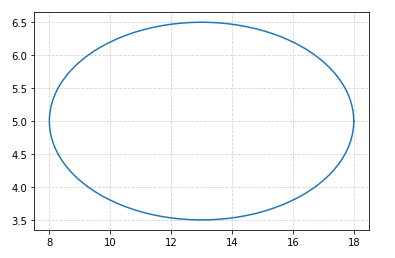
\includegraphics[width=\columnwidth]{ellipse.png}
    \caption{Ellipse}
    \label{Ellipse along given axis}
\end{figure}


\end{document}